\lecture{9}{28. April 2026}{The Design of Feedback Control Systems}

\section{The Design of Feedback Control Systems}

\subsection{Introduction and Concepts}
Often, it is not enough to only adjust one system parameter.
For example, suppose your motor system is too slow, overshoots too much, or has steady-state error.
You might try increasing the gain $K$, to make the response faster, however this will, in turn, create more overshoot thereby worsening one of the other problems.

To alleviate this, a compensator might be added.
Such a component can either be electrical, mechanical, hydraulic, pneumatic, or even purely software-based.
A compensator is often just written as a transfer function $G_c(s)$, implemented digitally or analogically.
The compensator transfer function is defined as all other transfer functions as
\begin{equation*}
  G_c(s) = \frac{E_o (s)}{E_{\mathrm{in}}(s)}
.\end{equation*}

The diagrams on \Cref{fig:comptype} depict different places where the compensator can be inserted.

\begin{figure} [ht]
  \centering
  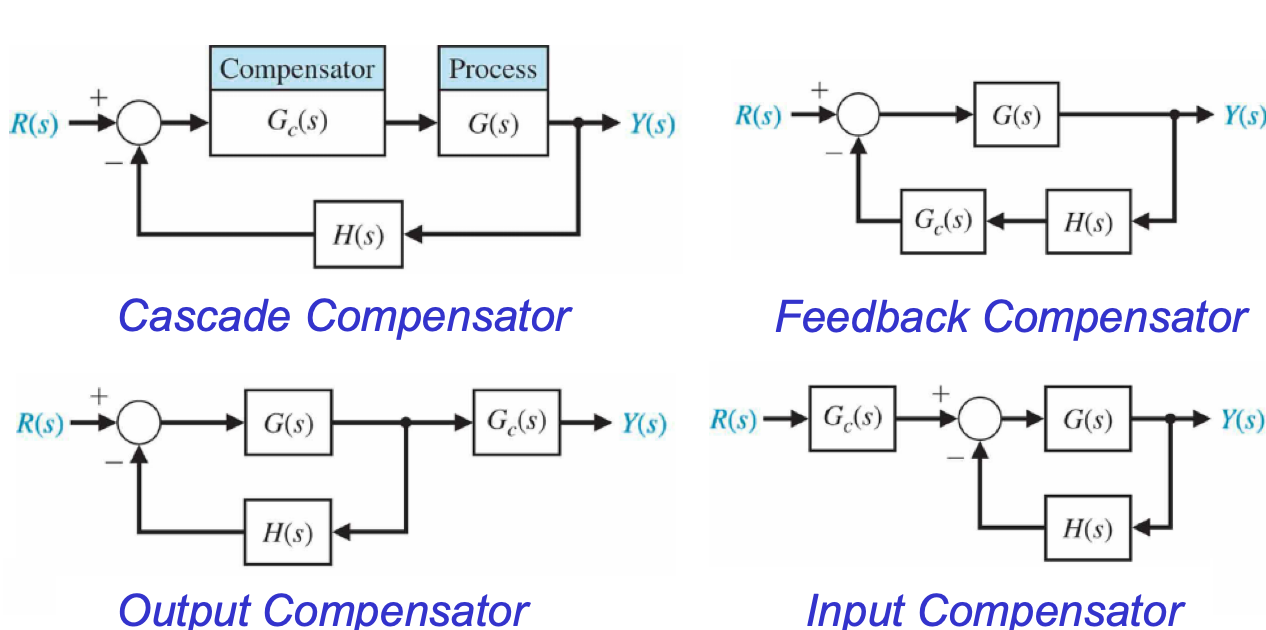
\includegraphics[width=0.8\linewidth]{./figures/comptype.png}
  \caption{Different types of compensator placements.}
  \label{fig:comptype}
\end{figure}

The most common form of a compensator is a cascade compensator, which is just placed in series with the plant.
In this case, the loop transfer function becomes:
\begin{equation*}
  L(s) = G_c(s) G(s) H(s)
.\end{equation*}

Another option is the feedback controller, where you are modifying the feedback signal before it is compared with the reference.
This can be useful if you want to shape sensor dynamics, filter feedback or change how the output is fed back, but it is usually less intuitive than a cascade controller.

One may also place the compensator after the plant output, thereby creating an output compensator, meaning the feedback loop may regulate an internal signal and then $G_c(s)$ modifies the final output signal.
This can be useful for output filtering or signal shaping, but it doe not affect the main feedback loop in the same direct way as a cascade or feedback compensator does.

Placing the compensator before the summing junction acting on the reference input creates an input compensator, which is essentially a prefilter.
It changes how the command enters the system, but it does not directly change the feedback loop stability.
E.g. one might choose to smooth a step input before feeding it to the controller so the motor does not get a harsh command. 

There are two major classical design approaches in this field.
The first of these is the root locus method, which focuses on the closed-loop poles, as these determine much of the transient response.
This is especially connected to time-domain specs such as settling time, overshoot, damping ratio and natural frequency.

The other major method is the frequency response method, which uses Bode plots.
Instead of directly looking at pole movement, you instead reshape the magnitude and phase of the loop transfer function.
This lets you tune things like bandwidth, phase margin, gain margin, and noise sensitivity.

The general form of a compensator is
\begin{equation*}
  G_c(S) = \frac{K \prod_{i = 1}^{M} (s + z_i)}{\prod_{j = 1}^{n} \left( s + p_j \right)}
.\end{equation*}
Meaning the compensator is representable by a gain $K$, zeros at $s = -z_i$ and poles at $s = - p_j$.
The design problem then becomes choosing appropriate values of $K, z_i, p_j$ to obtain the desired closed-loop system behaviour.

From the above, the simplest compensator is a so-called first-order compensator:
\begin{equation*}
  G_c(s) = \frac{K(s +z)}{s + p}
.\end{equation*}
This has one zero at $s = -z$, one pole at $s = -p$ and a gain $K$.
So here, the design problem is simply choosing a value of $K, z,p$.

\subsection{Phase-Lead Compensation}
From above, the basic form  of a first-order compensator is
\begin{equation*}
  G_c(s) = \frac{K(s+z)}{s+p}
.\end{equation*}
For a phase-lead compensator, the zero is closer to the origin than the pole, i.e. $\left| z \right| < \left| p \right|$ or, since $z$ and $p$ are positive constants $z < p$. This is shown on the pole-zero plot on \Cref{fig:phase_lead}.

\begin{figure} [ht]
  \centering
  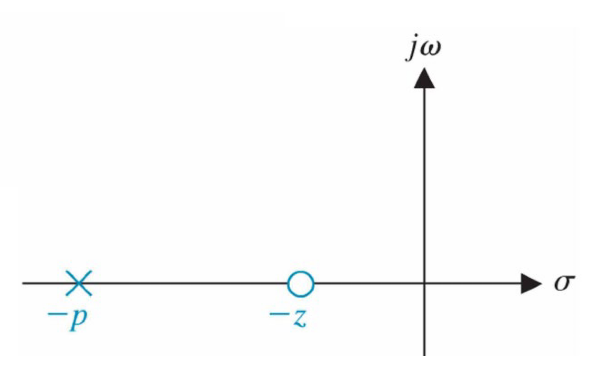
\includegraphics[width=0.8\linewidth]{./figures/phase_lead.png}
  \caption{Pole-zero plot for a phase-lead compensator.}
  \label{fig:phase_lead}
\end{figure}

A phase-lead compensator adds positive phase over some frequency range, thereby making the system behave as if it has less delay.
This is very useful as phase lead can improve the phase margin and thereby improve stability margin, damping, overshoot, and speed.
So a phase-lead compensator is usually used when the system is too sluggish, too oscillatory, or has too little phase margin.

We can rewerite
\begin{equation*}
  G_c (j \omega) = \frac{K (j\omega + z)}{j\omega + p}
\end{equation*}
in a more useful frequency-response form.
We start by factoring $p$ and $z$ as:
\begin{equation*}
  G_c(j\omega) = \frac{K z}{p}\frac{1 + j \frac{\omega}{z}}{1 + j \frac{\omega}{p}}
.\end{equation*}
Then, we define $\alpha = p / z$, so for phase lead $\alpha > 1$. 
We also define $\tau = 1 / p$, and since $p = \alpha z$ we get $1 / z = \alpha \tau$.
Therefore
\begin{equation*}
  G_c (j\omega) = K_1 \frac{1 + j\alpha \omega \tau}{1 + j\omega\tau}, \quad K_1 = \frac{K}{\alpha} \quad \alpha > 1
.\end{equation*}
This is the standard lead-compensator form.

\subsubsection{Bode Plot of a Phase-Lead Compensator}
The Bode plot on \Cref{fig:phaseleadbode} depicts the magnitude and phase as functions of frequency for the standard phase-lead compensator.
For the normalized lead compensator
\begin{equation*}
  \frac{G_c(j\omega)}{K_1} = \frac{1 + j\alpha \omega \tau}{1 + j\omega\tau}
\end{equation*}
the zero occurs at
\begin{equation*}
  \omega = z = \frac{1}{\alpha \tau}
\end{equation*}
and the pole occurs at
\begin{equation*}
  \omega = p = \frac{1}{\tau}
.\end{equation*}
Since $\alpha > 1$, the zero comes before the pole:
\begin{equation*}
  \frac{1}{\alpha \tau} < \frac{1}{\tau}
.\end{equation*}
Which is why the magnitude plot is flat at low frequencies, then rises with slope \qty{20}{\dB/dec} between the zero and pole and then flattens out again.
The high-frequency gain increase is $20 \log \alpha$, which is the aforementioned extra high-frequency gain caused by a lead compensator.
Therefore a phase-lead compensator may be very useful for improving speed and bandwidth, but it can also start to amplify high-frequency noise if overdone.

\begin{figure} [ht]
  \centering
  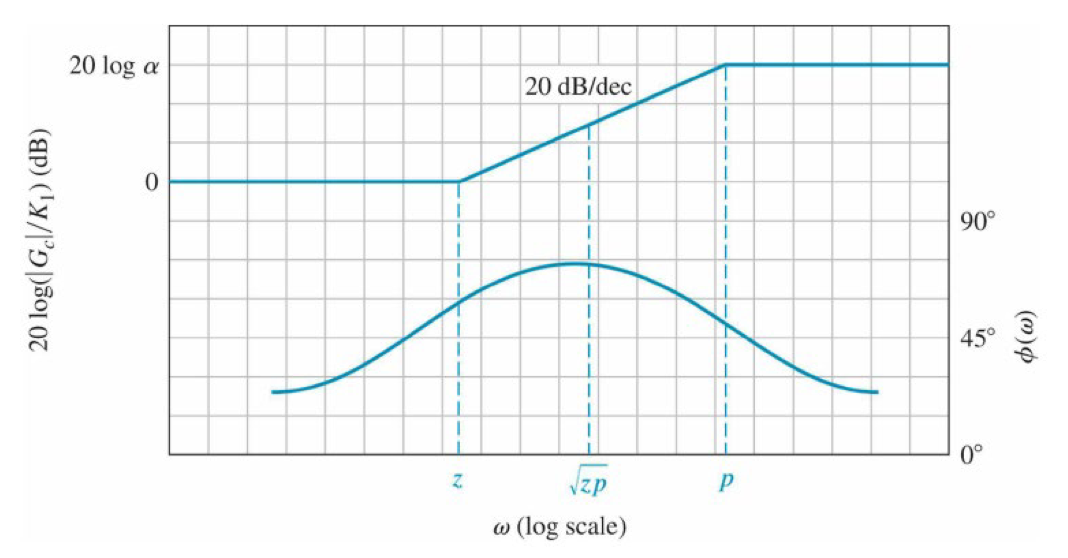
\includegraphics[width=0.8\linewidth]{./figures/phaseleadbode.png}
  \caption{Bode plot of a phase-lead compensator.}
  \label{fig:phaseleadbode}
\end{figure}

The phase angle of the lead compensator on \Cref{fig:phaseleadbode} is given by
\begin{equation*}
  \phi (\omega) = \tan^{-1}(\alpha\omega\tau) - \tan^{-1}(\omega\tau)
.\end{equation*}
The numerator zero contributes positive phase, and the denominator pole contributes negative phase, but because the zero happens first, the positive phase contribution appears before the negative pole contribution catches up.
So for a range of frequencies $\phi(\omega) > 0$; that is the phase lead.
The curve rises, reaches a maximum, and then falls back toward zero.

The maximum phase lead occurs halfway between the zero and the pole on a logarithmic frequency scale:
\begin{equation*}
  \omega_m = \sqrt{zp} = \frac{1}{\tau \sqrt{\alpha}}
.\end{equation*}
This is very important in compensator design.
Usually, you place $\omega_m$ near the desired gain crossover frequency, as that is where we want the most extra phase margin.

We also have that
\begin{equation*}
  \sin \phi_m = \frac{\alpha-1}{\alpha + 1} 
\end{equation*}
which tells how much maximum phase lead you get from a chosen pole-zero ratio $\alpha$.
This can also be solved as
\begin{equation*}
  \alpha = \frac{1 + \sin \phi_m}{1 - \sin \phi_m}
\end{equation*}
so if you know how much extra phase you need, you can calculate the required $\alpha$.
In theory, as $\alpha \to \infty$, the phase lead approaches \ang{90}, as shown on \Cref{fig:phaseangmax}.

\begin{figure} [ht]
  \centering
  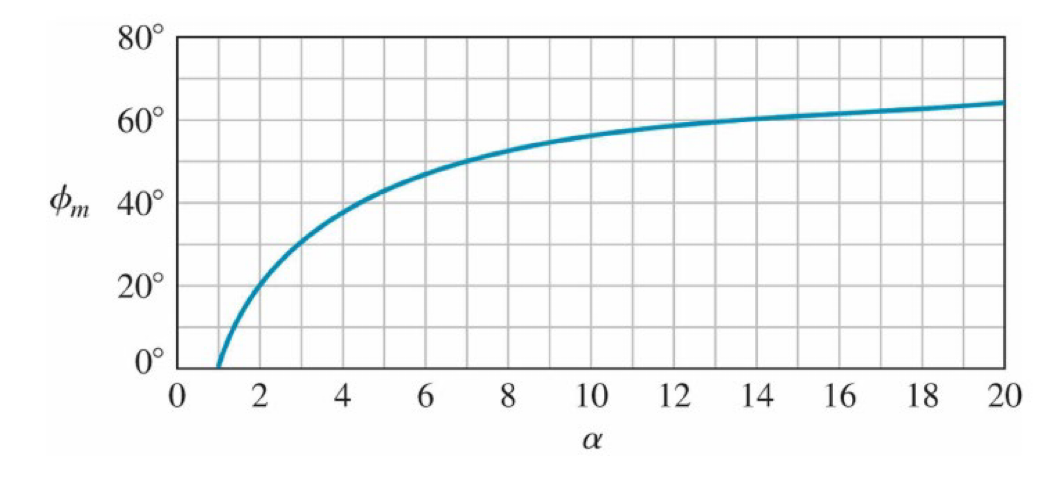
\includegraphics[width=0.8\linewidth]{./figures/phaseangmax.png}
  \caption{Maximum phase lead $\phi_m$ and pole-zero ratio $\alpha$}
  \label{fig:phaseangmax}
\end{figure}


However, in practice, single lead stages are usually kept below roughly \qtyrange{60}{70}{\degree}, because large $\alpha$ give too much gain boost and noise sensitivity.
If more phase lead is needed, you normally use two lead compensators instead of one extreme one.one extreme one.


\begin{figure} [ht]
  \centering
  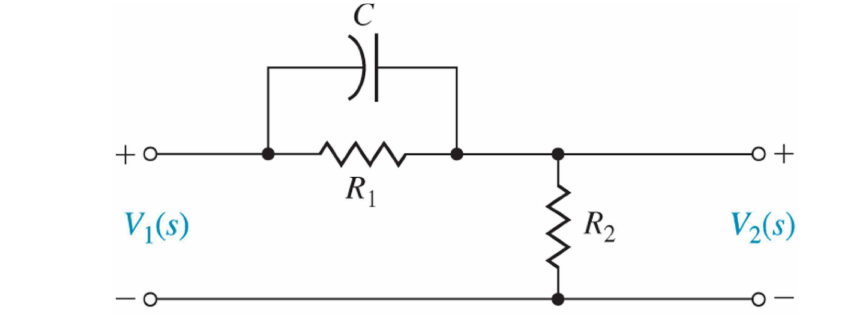
\includegraphics[width=0.5\linewidth]{./figures/phaseleadrc.png}
  \caption{Simple RC-realization of a phase-lead compensator.}
  \label{fig:phaseleadrc}
\end{figure}

The RC-network on \Cref{fig:phaseleadrc} realizes the transfer function
\begin{equation*}
  G_c(s) = \frac{1 + \alpha \tau s}{\alpha (1 + \tau s)}
.\end{equation*}
The important part here is not the exact circuit algebra, but the structure.
For the circuit shown:
\begin{equation*}
  \tau = \frac{R_1 R_2}{R_1 + R_2} C
\end{equation*}
and
\begin{equation*}
  \alpha = \frac{R_1 + R_2}{R_2}
.\end{equation*}
Since $R_1 + R_2 > R_2$, we get $\alpha > 1$, which is the condition for phase lead.
As the circuit is passive, it also includes attenuation, hence the $1 / \alpha$ factor in front of the transfer function.


\subsection{Phase-Lag Compensation}
The transfer function for a phase-lag compensator is normally written as
\begin{equation*}
  G_c (s) = \frac{1 + \tau s}{1 + \alpha \tau s}
\end{equation*}
with $\alpha > 1$.
The above can also be written as
\begin{equation*}
  G_c (s) = \frac{1}{\alpha} \frac{s + z}{s + p}
.\end{equation*}
Where $z = 1 / \tau$ and $p = 1 / \alpha \tau$.
Since $\alpha > 1$, $p < z$, so the pole is closer to the origin than the zero as shown on \Cref{fig:phaselagpz}.

\begin{figure} [ht]
  \centering
  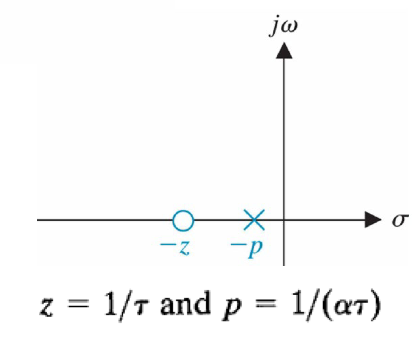
\includegraphics[width=0.5\linewidth]{./figures/phaselagpz.png}
  \caption{Pole-zero plot for a phase-lag compensator}
  \label{fig:phaselagpz}
\end{figure}

A phase-lag compensator adds negative phase over some frequency range.
This seems contrary to our goal of stability as this seemingly decreases phase margin, however phase-lag compensators are mainly used to improve steady-state accuracy without strongly changing the crossover frequency.
This is because a lag-compensator can increase the effective low-frequency gain compared with high-frequency gain, which helps reduce steady-state error.

A phase-lag network behaves like an integrator over a finite range of frequencies.
An ideal integrator has transfer function $1 / s$ and gives \qty{-20}{\dB/dec} with phase \ang{-90}.
A lag-compensator is not a true integrator, but between its pole and zero, its Bode magnitude falls with approximately \qty{-20}{\dB/dec}  and its phase becomes negative.
So in this way a phase-lag compensator behaves integrator-like over a limited frequency range.

\subsubsection{Bode Plot of a Phase-Lag Compensator}
The Bode plot for lag compensation, shown on \Cref{fig:phaselagbode} is basically the mirror image of the phase-lead case.
The pole comes first at
\begin{equation*}
  \omega = p = \frac{1}{\alpha \tau}
\end{equation*}
and then the zero comes later
\begin{equation*}
  \omega = z = \frac{1}{\tau}
\end{equation*}
so the magnitude starts flat, then drops \qty{-20}{\dB/dec}, between the pole and the zero and then becomes flat again at a lower gain.

\begin{figure} [ht]
  \centering
  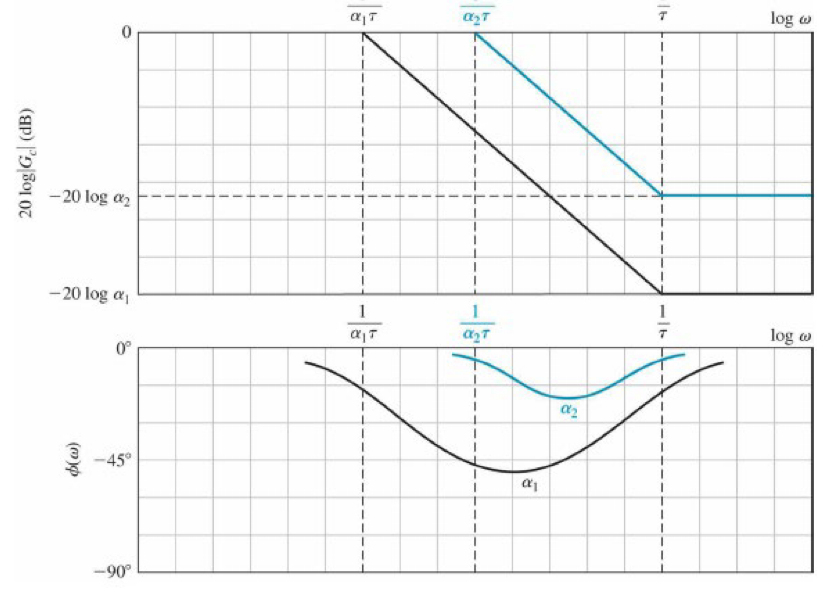
\includegraphics[width=0.8\linewidth]{./figures/phaselagbode.png}
  \caption{Bode plot of a phase-lag compensator}
  \label{fig:phaselagbode}
\end{figure}

The phase becomes negative between the pole and zero on \Cref{fig:phaselagbode}, and the maximum phase lag occurs at
\begin{equation*}
  \omega_m = \sqrt{zp}
\end{equation*}
just like the lead case, but now it is a maximum negative phase angle instead of a positive one.

\subsection{Phase-Lead Design}
In the following we will be going through the phase-lead design process first through the Bode diagram method in \Cref{sec:pldbd} and then the root locus method in \Cref{sec:pldrl} through two worked examples.

\subsubsection{Phase-Lead Design Using the Bode Diagram} \label{sec:pldbd}
The overall goal in the following section is to take an uncompensated system with poor stability margin and add a compensator $G_c(s)$ to give extra positive phase near the gain crossover frequency.

The general Bode design procedure in this context is to
\begin{enumerate}
  \item start with the uncompensated open-loop system,
  \item check its current phase margin,
  \item decide how much extra phase is needed,
  \item choose $\alpha$ from the required phase lead,
  \item plade the compensator zero and pole around the new crossover frequency
  \item check the final Bode plot.
\end{enumerate}
The important trick here is that at the frequency of maximum phase lead, the compensator adds a magnitude boost of $10 \log \alpha$, so if we want the new crossover to happen at $\omega_n$, you simply choose $\omega_m$, where the uncompensated magnitude is $-10 \log \alpha \, \unit{\dB}$.
Then once the compensator adds $10 \log \alpha$, the magnitude becomes \qty{0}{\dB} and that frequency becomes the new gain crossover frequency.

\begin{figure} [ht]
  \centering
  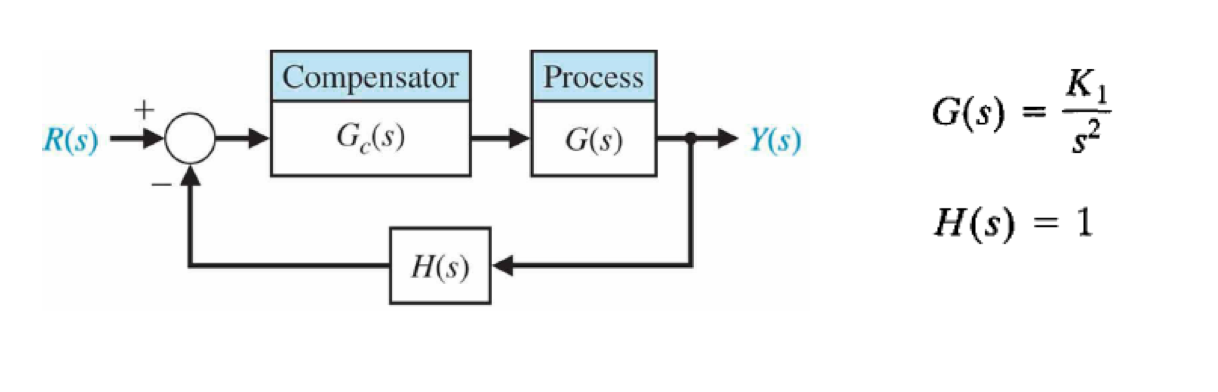
\includegraphics[width=0.6\linewidth]{./figures/phasebodeex.png}
  \caption{Example system for Bode-phase-lead design.}
  \label{fig:phasebodeex}
\end{figure}
We consider the system on \Cref{fig:phasebodeex} with $G(s) = K_1 / s^2$ and $H(s) = 1$.
This is a type-two system as the open-loop transfer function has two pure integrators $1 / s^2$.
The specifications are a settling time $T_s \leq \qty{4}{\s}$ and a damping constant $\xi \geq \num{0,45}$.

Without the compensator the closed loop transfer function of the system on \Cref{fig:phasebodeex} is
\begin{equation*}
  T(s) = \frac{Y(s)}{R(s)} = \frac{K_1}{s^2 + K_1}
.\end{equation*}
Comparing this with the standard second order form:
\begin{equation*}
  T(s) = \frac{\omega_n^2}{s^2 + 2\xi \omega_n  + \omega_n^2}
\end{equation*}
i.e. $2 \xi \omega_n = 0 \implies \xi = 0$, so the system is unddampened and the poles are purely imaginary $s = \pm j \sqrt{K_1}$.
This means the system oscillates without settling properly, and since the system is undamped the requirements are not fulfilled.
Changing $K_1$ alone changes the natural frequency, but it doe not add damping.

For a second-order system, our settling time is given as:
\begin{equation*}
  T_s \approx \frac{4}{\xi \omega_n}
.\end{equation*}
We require $T_s \leq 4$ and $\xi \geq \num{0,45}$ so
\begin{equation*}
  4 \geq \frac{4}{\num{0,45} \omega_n} \implies \omega_n \geq \frac{1}{\num{0,45}} = \qty{2,22}{rad\per\s} 
.\end{equation*}

\begin{figure} [ht]
  \centering
  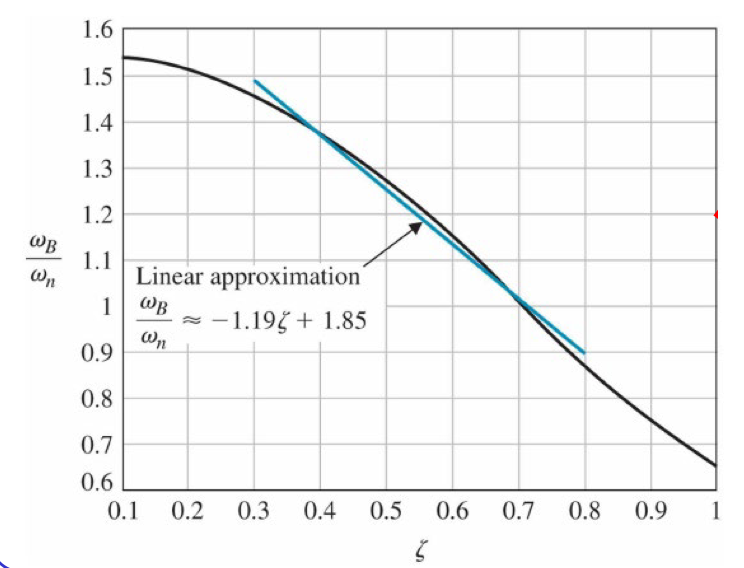
\includegraphics[width=0.5\linewidth]{./figures/bandwidthbode.png}
  \caption{Closed-loop bandwidth $\omega_B$ compared to natural frequency $\omega_n$}
  \label{fig:bandwidthbode}
\end{figure}
For $\xi = \num{0,45} $, \Cref{fig:bandwidthbode} gives approximately:
\begin{align*}
  \frac{\omega_B}{\omega_n} &\approx \num{1,33} \\
  \omega_B &= \num{1,33} \omega_n \\
  &= \num{1,33} \cdot \qty{2,22}{rad\per\s}  \\
  &= \qty{3,0}{rad\per\s} 
.\end{align*}
So the closed-loop bandwidth of the system should be roughly $\omega_B \approx \qty{3,0}{rad\per\s}$.

For the uncompensated system,
\begin{equation*}
  T(s) = \frac{K_1}{s^2 + K_1}
\end{equation*}
so $\omega_n = \sqrt{K_1}$.
From $\omega_B = \num{1,33} \omega_n \geq \qty{3,0}{rad\per\s}$ we see that $K_1 = 5$ is enough for the bandwidth, but we opt for $K_1 = 10$ to provide a safety margin.
So the uncompensated open-loop transfer function becomes
\begin{equation*}
  G(s) = \frac{10}{s^2}
\end{equation*}
but thi still has a phase of \ang{-180} at all frequencies because
\begin{equation*}
  \frac{1}{\left( j\omega \right)^2} = - \frac{1}{\omega^2}
\end{equation*}
so the phase margin is zero.
The gain is therefore now large enough, but the damping/stability margin is still not acceptable.

The required damping ratio is $\xi \geq \num{0,45}$.
A rough design rule is that $\xi \approx \num{0,01} \phi_{pm}$, where $\phi_{pm}$ is in degrees.
So
\begin{equation*}
  \phi_{pm} \approx \frac{\xi}{\num{0,01}} = \frac{\num{0,45} }{\num{0,01}} = \ang{45} 
.\end{equation*}
The uncompensated system has approximately zero phase margin, so the compensator should add roughly \ang{45} of phase lead.

The maximum phase lead is given by
\begin{equation*}
  \sin \phi_m = \frac{\alpha - 1 }{\alpha + 1}
.\end{equation*}
Here $\phi_m = \ang{45}$, so
\begin{equation*}
  \sin \ang{45} = \frac{\alpha - 1}{\alpha + 1} \implies \alpha \approx \num{5,8} 
.\end{equation*}
We choose $\alpha = 6$ to provide a little safety margin.

Now we find the new crossover frequency by computing $10 \log \alpha$ with $\alpha = 6$, we get
\begin{equation*}
  10 \log 6 = \qty{7,78}{\dB} 
.\end{equation*}
The design rule says to find the frequency, where the uncompensated magnitude is \qty{-7,78}{\dB}.
For the uncompensated open-loop system:
\begin{equation*}
  G(j\omega) = \frac{10}{\left( j\omega \right)^2}
.\end{equation*}
The magnitude is
\begin{equation*}
  \left| G(j\omega) \right| = \frac{10}{\omega^2}
.\end{equation*}
Or in \unit{\dB}:
\begin{equation*}
  20 \log \left| G(j\omega) \right| = 20 \log \left( \frac{10}{\omega^2} \right)
.\end{equation*}
This equals \qty{-7,78}{\dB} at about $\omega_n = \qty{4,95}{rad\per\s}$.
So we place the maximum phase lead at $\omega_m = \qty{4,95}{rad\per\s}$.

For a lead compensator:
\begin{equation*}
  \omega_m = \sqrt{zp}
.\end{equation*}
and
\begin{equation*}
  \alpha = \frac{p}{z}
.\end{equation*}
So
\begin{align*}
  p &= \omega_m \sqrt{a} \\
  z &= \frac{p}{\alpha}
.\end{align*}
Using
\begin{align*}
  \omega_m &= \num{4,95}  \\
  \alpha &= 6
.\end{align*}
Gives
\begin{equation*}
  p = \num{4,95} \sqrt{6} \approx \num{12,0}  \qquad z = \frac{\num{12,0} }{6} = \num{2,0} 
.\end{equation*}
So the compensator zero is at $s = -2$ and the compensator is at $s = -12$. 
Using the pole and zero values the lead compensator can be written as
\begin{equation*}
  G_c(s) = \frac{1 + \frac{s}{2}}{1 + \frac{s}{12}} = \frac{6(s + 2)}{s + 12}
.\end{equation*}

The uncompensated plant was
\begin{equation*}
  G(s) = \frac{10}{s^2}
\end{equation*}
and the compensator is
\begin{equation*}
  G_c(s) = \frac{1 + \frac{s}{2}}{1 + \frac{s}{12}}
,\end{equation*}
so the compensated loop transfer function is:
\begin{align*}
  L(s) &= G_c(s) G(s) \\
  &= \frac{10}{s^2} \frac{1 + \frac{s}{2}}{1 + \frac{s}{12}} \\
  &= \frac{60 ( s + 2)}{s^2 (s + 12)}
.\end{align*} 
For unity feedback,
\begin{equation*}
  T(s) = \frac{L(s)}{1 + L(s)}  = \frac{60 (s+2)}{s^3 + 12s^2 + 60s + 120} \approx \frac{60 (s + 2)}{\left( s^2 + 6s + 20 \right) \left( s + 6 \right)}
.\end{equation*}
The dominant second-order part is approximately $s^2 + 6s + 20$.
Comparing this with the standard second-order form $s^2 + 2\xi \omega_n s + \omega_n^2$, we see that $\omega_n = \num{4,47}$ and $\xi \approx \num{0,67}$.
Hence, the damping ratio $\xi \approx \num{0,67} \geq \num{0,45} $ exceeds the requirement.
The approximate settling time is
\begin{equation*}
  T_s \approx \frac{4}{\xi \omega_n} = \frac{4}{\num{0,67} \cdot \num{4,47}} = \qty{1,34}{\s} 
.\end{equation*}
So the requirement for the settling time $T_s \leq \qty{4}{\s}$ is also satisfied.

\begin{figure} [ht]
  \centering
  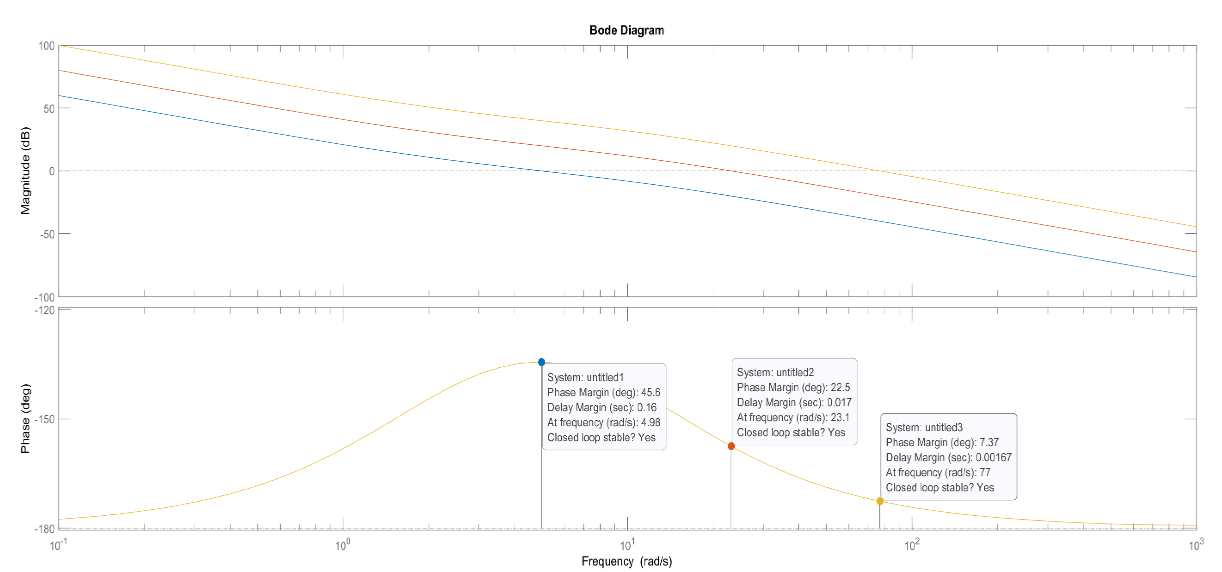
\includegraphics[width=0.75\linewidth]{./figures/bodefinal.png}
  \caption{Bode plot for the compensated loop transfer function.}
  \label{fig:bodefinal}
\end{figure}

On \Cref{fig:bodefinal} the Bode plots for the compensated loop transfer function is shown.
The phase margin here is roughly \ang{45,6} at around $\omega \approx \qty{4,98}{rad\per\s} $, that matches the design goal of $\phi_{pm} = \ang{45}$ almost exactly.


\subsubsection{Phase-Lead Design using Root Locus} \label{sec:pldrl}
The overall goal here, is to choose $G_c(s)$ so that the closed-loop poles move to a desired location in the $s$-plane.
For this example we will continue working with the system from before with $G(s) = K_1 / s^2$ and unity feedback as depicted on \Cref{fig:phaserlex}.

\begin{figure} [ht]
  \centering
  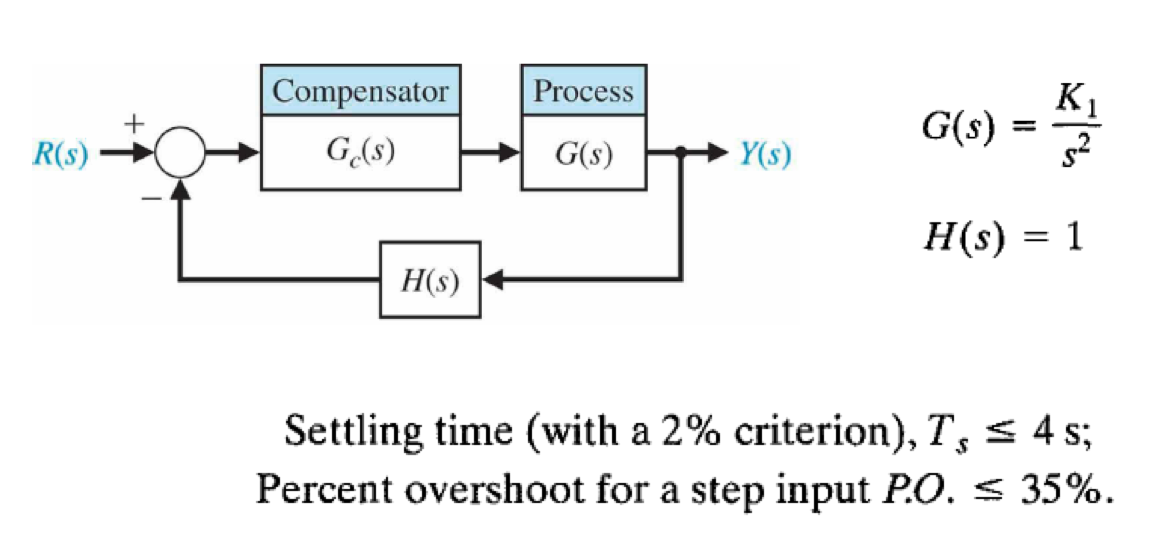
\includegraphics[width=0.8\linewidth]{./figures/phaserlex.png}
  \caption{Example system for root locus phase-lead design.}
  \label{fig:phaserlex}
\end{figure}

The compensator is chosen as a first-order lead compensator:
\begin{equation*}
  G_c(s) = \frac{s+z}{s+p}
.\end{equation*}
For phase lead, we have that $\left| z \right| < \left| p \right|$, so the zero is closer to the origin than the pole.
The purpose of adding this pole-zero pair is to reshape the root locus so that it passes through the desired closed-loop pole location.

The general root-locus design recipe is, to start from performance requirements, e.g.:
\begin{gather*}
  T_s \leq \qty{4}{\s} \\
  P.O. \leq 35\%
.\end{gather*}
Then you translate those into a desired dominant pole location:
\begin{equation*}
  s_d = -\sigma \pm j\omega_d
\end{equation*}
where the real part $-\sigma$ controls the settling speed, and the imaginary part $\omega_d$ controls oscillation frequency.
Then, you
\begin{enumerate}
  \item draw the uncompensated root locus,
  \item check whether the desired point lies on it,
  \item if not, add a phase-lead compensator,
  \item place the compensator zero,
  \item choose the compensator pole so that the angle condition is satisfied,
  \item compute the required gain using the magnitude condition.
\end{enumerate}
The root locus condition is
\begin{equation*}
  1 + L(s) = 0
\end{equation*}
so the point on the root locus must satisfy
\begin{equation*}
  \angle L(s) = \left( 2k + 1 \right) \ang{180}
\end{equation*}
and $\left| L(s) \right| = 1$.
The angle condition tells you where the pole and zero should go, and the magnitude condition tells you the required gain.

The root locus is prepared as explained in \Cref{sec:rlmethod}, however, for completenes, the most important rules will be reiterated here.
First of all, the root locus starts at open-loop poles and ends at open-loop zeros.
If there are more poles than zeros, some branches go to infinity.
The number of branches is equal to the number of open-loop poles.
The locus is symmetric about the real axis.
On the real axis, the root locus exists to the left of an odd number of real poles and zeros.
For poles going to infinity, the asymptote centroid is:
\begin{equation*}
  \sigma_A = \frac{\sum \text{poles} - \sum \text{zeros}}{n - M}
\end{equation*}
and the asymptote angles are
\begin{equation*}
  \phi_A = \frac{\left( 2 k + 1 \right) \ang{180} }{n -M}
.\end{equation*}

As mentioned above and on \Cref{fig:phaserlex}, the example system is $G(s) = K_1 / s^2, H(s) = 1$, where we require $T_s \leq \qty{4}{\s}$ and $P.O. \leq 35\%$.
Currently, the poles of the closed-loop system are $s = \pm j \sqrt{K_1}$, so the closed-loop poles are purely imaginary.
That means the root locus lies on the $j\omega$-axis, meaning the uncompensated system is undamped and does not meet the requirements.

The overshoot requirement is $P.O. \leq 35\%$.
For a second-order system, overshoot is related to damping ratio $\xi$.
A 35\% overshoot corresponds roughly to $\xi \geq \num{0,32}$.
The settling-time requirement is
\begin{equation*}
  T_s \approx \frac{4}{\xi \omega_n} \implies \xi \omega_n \geq 1
.\end{equation*}
We choose the desired dominant roots as $s_d = -1 \pm j2$.
For this point:
\begin{equation*}
  \omega_n = \sqrt{1^2 + 2^2} = \sqrt{5} \approx \num{2,23} 
\end{equation*}
and
\begin{equation*}
  \xi = \frac{1}{\sqrt{5}} \approx \num{0,45} 
.\end{equation*}
So this chosen point satisfies both requirements
\begin{equation*}
  \xi = \num{0,45} > \num{0,32} 
\end{equation*}
and $T_s \approx 4 / (\num{0,45} \cdot \num{2,23} ) \approx 4$, so the desired dominant closed-loop poles are:
\begin{equation*}
  s = -1 \pm j2
.\end{equation*}
We choose to place the compensator zero directly below the desired root location, meaning the compensator zero is places at $s = -1 \implies z = 1$.
So at this point
\begin{equation*}
  G_c(s) = \frac{s + 1}{s + p}
.\end{equation*}
We still need to find the compensator pole $p$.

Now, we need the desired point $s_d = -1 +j2$ to lie on the compensated root locus.
The compensated transfer function will be:
\begin{equation*}
  L() = \frac{K_1(s + 1)}{s^2 (s + p)}
.\end{equation*}
The angle condition says that $\angle L(s_d) = \ang{-180}$.
The contributions come from two poles at the origin, one zero at $-1$, and one unknown pole at $-p$.
At the desired point, the angle from each pole to the origin is about \ang{116}.
There are two of them, so the pole contribution from these is \ang{-232}.
The zero at $-1$ points vertically upward to the desired point, so its angle contribution is \ang{90}.
Therefore without the unknown pole:
\begin{equation*}
  \phi = \ang{-232} + \ang{90} = \ang{-142}
.\end{equation*}
So the missing pole contribution must be
\begin{equation*}
  \ang{-180} = \ang{-142} - \theta_p \implies \theta_p = \ang{38} 
.\end{equation*}
So we draw a line from the desired root location at an angle of \ang{38} down to the real axis as shown on \Cref{fig:rlex1}.
This line intersects the real axis at approximately $s = -\num{3,6} \implies p = \num{3,6}$.

\begin{figure} [ht]
  \centering
  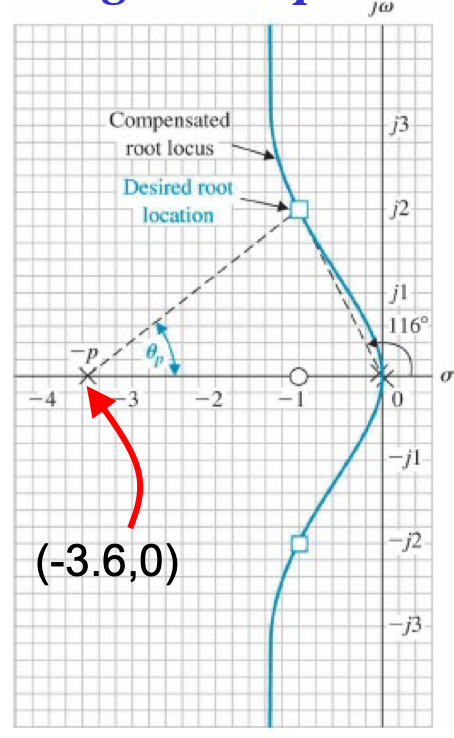
\includegraphics[width=0.3\linewidth]{./figures/rlex1.png}
  \caption{Compensated root locus with desired root locations and location of pole.}
  \label{fig:rlex1}
\end{figure}

So the compensator is
\begin{equation*}
  G_c(s) = \frac{s+1}{ s+ \num{3,6} }
.\end{equation*}
As $1 < \num{3,6}$, this is a phase-lead compensator.
The compensated loop transfer function is then:
\begin{align*}
  L(s) &= G_c(s) G(s) \\
       &= \frac{K_1 (s+1)}{s^2 (s + \num{3,6})}
.\end{align*}
Now the root locus has been reshaped so that it passes through the desired point $s = -1 \pm j 2$.

Now that the desired pole location lies on the root locus, the gain is found from the magnitude condition
\begin{equation*}
  \left| L(s_d) \right| = 1
.\end{equation*}
Using
\begin{equation*}
  L(s) = \frac{K_1 (s + 1)}{s^2 (s + \num{3,6} )}
\end{equation*}
we get
\begin{equation*}
  K_1 = \frac{\left| s_d \right|^2 \left| s_d + \num{3,6}  \right|}{\left| s_d + 1 \right|}
.\end{equation*}
At $s_d = -1 \pm j2$, we have
\begin{gather*}
  \left| s_d \right| = \sqrt{\left( -1 \right)^2 + 2^2} = \sqrt{5} = \num{2,23}  \\
  \left| s_d + \num{3,6}  \right| = \left| \num{2,6} + j2 \right| \approx \num{3,25} \\
  \left| s_d + 1 \right| = \left| j2 \right| = 2
.\end{gather*}
So 
\begin{equation*}
  K_1 = \frac{\left( \num{2,23}  \right)^2 \left( \num{3,25}  \right)}{2} \approx \num{8,1} 
.\end{equation*}
Therefore, the final open-loop compensated transfer function is
\begin{equation*}
  L(s) = \frac{\num{8,1} (s + 1)}{s^2 \left( s + \num{3,6}  \right)}
.\end{equation*}

Because the open-loop transfer function still has two integrators, this is still a type-two system.
The acceleration error constant is
\begin{equation*}
  K_a = \lim_{s \to 0}s^2 L(s) = \frac{\num{8,1} \cdot 1}{\num{3,6}} = \num{2,25} 
.\end{equation*}
So the parabolic-input steady-state error would be $e_{ss} = 1 / K_a \approx \num{0,44} $.


\begin{figure} [ht]
  \centering
  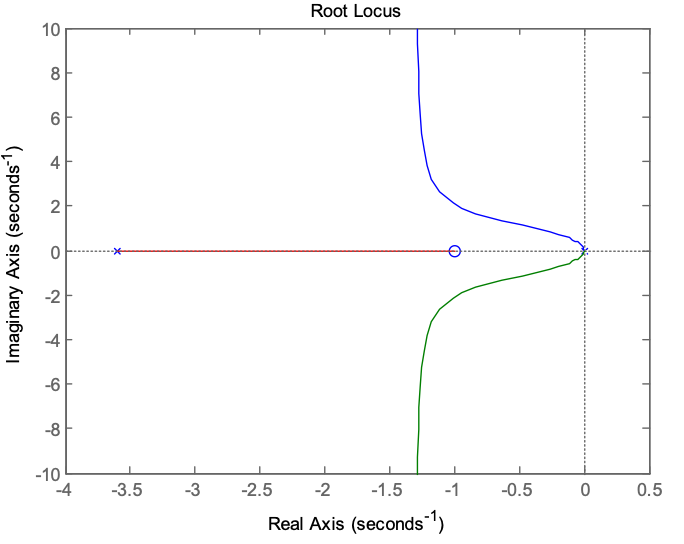
\includegraphics[width=0.6\linewidth]{./figures/rlfinal.png}
  \caption{Final root-locus plot for the example system.}
  \label{fig:rlfinal}
\end{figure}

The final root-locus plot for the example system is shown on \Cref{fig:rlfinal}.
